\documentclass[11pt,a4paper]{article}

\usepackage[margin=2.2cm]{geometry}
\usepackage{amsmath,amssymb}
\usepackage[T1]{fontenc}
\usepackage{lmodern}
\usepackage{microtype}
\usepackage{enumitem}
\usepackage[hidelinks]{hyperref}
\usepackage{xcolor}
\usepackage{tikz}
\usepackage{listings}
\usepackage{booktabs}
\usepackage{multirow}
\usetikzlibrary{positioning,arrows.meta,shapes.geometric,fit,calc}

\definecolor{deepblue}{RGB}{30,80,150}
\definecolor{deepgreen}{RGB}{40,120,60}
\definecolor{deepred}{RGB}{170,50,50}
\definecolor{soft}{RGB}{220,225,235}
\definecolor{warn}{RGB}{200,120,40}
\definecolor{kept}{RGB}{40,140,80}
\definecolor{cut}{RGB}{170,60,60}

\tikzset{
    tens/.style={ellipse,draw=deepblue,thick,fill=deepblue!10,minimum width=14mm,minimum height=6mm,inner sep=1pt,font=\scriptsize},
    layer/.style={rectangle,draw=deepgreen,thick,fill=deepgreen!10,rounded corners=2pt,minimum width=18mm,minimum height=7mm,inner sep=2pt,font=\scriptsize},
    box/.style={rectangle,draw=deepblue,thick,fill=soft,rounded corners=2pt,inner sep=4pt,font=\small},
    arr/.style={-{Stealth[length=2.2mm]},semithick},
}

\lstset{
    basicstyle=\ttfamily\small,
    breaklines=true,
    columns=fullflexible,
    keepspaces=true,
    showstringspaces=false,
    frame=single,
    framesep=3pt,
    rulecolor=\color{soft},
}

\newcommand{\HSiKAN}{\textsc{HSiKAN}}
\newcommand{\HyMeKo}{\textsc{HyMeKo}}
\newcommand{\code}[1]{\texttt{\small #1}}
\setlist[itemize]{leftmargin=1.4em,itemsep=2pt,topsep=3pt}

\title{\HyMeKo-driven \HSiKAN: \\[2pt]
       \large{\normalfont architecture, training, and three tuning expressions}}
\author{}
\date{2026-05-05}

\begin{document}
\maketitle

\noindent
This brief documents the overnight work: \HSiKAN{}'s architecture,
training loop, and tuning policies expressed as \HyMeKo{}
descriptions, with a Python driver that walks the parsed AST and
runs an actual training cell. The smoke test on
\code{bitcoin\_alpha} reproduces the hand-coded
$m{=}16,\ \text{pruner}{=}\text{davis}$ result (AUC 0.7930) starting
from \emph{nothing but} \code{.hymeko} files on disk.

% ────────────────────────────────────────────────────────────────────
\section{What landed}

Five concrete artefacts:

\begin{itemize}
\item \code{hymeko\_py::hymeko\_parse::parse\_hymeko\_rs} --- PyO3
      bridge wrapping \code{parser::parse\_description}; emits the
      AST as a nested Python dict.
\item \code{data/hsikan/arch\_single\_k3.hymeko} +
      \code{arch\_mixed\_k34.hymeko} --- HSiKAN architectures as
      per-layer hyperedges over tensor nodes.
\item \code{data/hsikan/training.hymeko} --- training/feedback
      dataflow (dataset $\to$ cycle\_enum $\to$ forward $\to$ loss
      $\to$ backward $\to$ optimizer + entropy regulariser).
\item \code{data/hsikan/sweep\_grid.hymeko} +
      \code{sweep\_genetic.hymeko} +
      \code{sweep\_msg.hymeko} --- three tuning policies (Cartesian
      grid, GA, P-graph axiom-feasibility).
\item \code{signedkan\_wip/src/hymeko\_driver.py} --- driver that
      parses, extracts knobs, and dispatches into the existing
      \code{run\_final\_cell.cell\_signed\_graph}.
\end{itemize}

% ────────────────────────────────────────────────────────────────────
\section{Schema}

\subsection{Tensors and layers as a hierarchical hypergraph}

Convention (matches
\code{transforms/torch\_dataflow/template.py}):

\begin{lstlisting}
// Tensors are nodes tagged by role.
t_in     <input>;
t_emb_k3 <activation>;
t_out    <output>;

// Layers inherit from a layer-class base; sub-tags are kwargs.
sk_k3 : signedkan_layer { hidden 16; arity 3; grid 5; spline_kind "catmull_rom"; }
mixer : arity_mixer     { hidden 16; mix_K 2; }
head  : signed_classifier { d_in 16; d_out 1; }

// Dataflow: @name <dataflow> { (+input, ~layer, -output); }
@flow_k3   <dataflow> { (+t_in,    ~sk_k3, -t_emb_k3); }
@flow_mix  <dataflow> { (+t_emb_k3, +t_emb_k4, ~mixer, -t_emb); }
@flow_head <dataflow> { (+t_emb,    ~head,  -t_out); }
\end{lstlisting}

Multi-input fan-in (the arity mixer) is one hyperedge with two
\code{+}-signed source tensors and one \code{-}-signed sink. The
template's \code{bind:+:all\_csv} renders this as a multi-arg call
in PyTorch.

\subsection{Mixed-arity HSiKAN as a HyMeKo dataflow graph}

\begin{center}
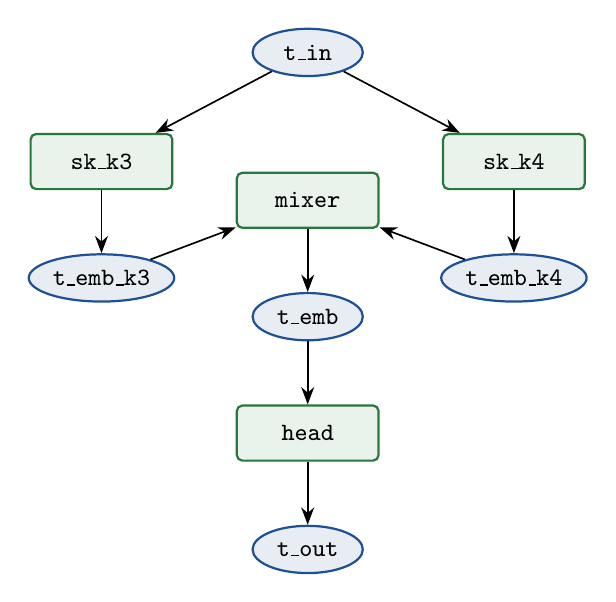
\begin{tikzpicture}[node distance=8mm and 12mm,every node/.style={font=\scriptsize}]
\node[tens]  (tin)   {\code{t\_in}};
\node[layer,below left=of tin]  (sk3)  {\code{sk\_k3}};
\node[layer,below right=of tin] (sk4)  {\code{sk\_k4}};
\node[tens,below=of sk3]  (e3)  {\code{t\_emb\_k3}};
\node[tens,below=of sk4]  (e4)  {\code{t\_emb\_k4}};
\node[layer,below=12mm of tin] (mix) {\code{mixer}};
\node[tens,below=of mix]  (e)  {\code{t\_emb}};
\node[layer,below=of e]   (h)  {\code{head}};
\node[tens,below=of h]    (out){\code{t\_out}};
\draw[arr] (tin) -- (sk3);
\draw[arr] (tin) -- (sk4);
\draw[arr] (sk3) -- (e3);
\draw[arr] (sk4) -- (e4);
\draw[arr] (e3)  -- (mix);
\draw[arr] (e4)  -- (mix);
\draw[arr] (mix) -- (e);
\draw[arr] (e)   -- (h);
\draw[arr] (h)   -- (out);
\end{tikzpicture}
\end{center}

Two parallel \code{signedkan\_layer}{} stacks (one per arity) feed
an \code{arity\_mixer} that learns the $\alpha_k$ mixture
weights. The driver reads this file and constructs the
\code{MixedAritySignedKAN} module with the right
\code{(arities=[3,4], hidden=16, grid=5, spline\_kind="catmull\_rom")}.

% ────────────────────────────────────────────────────────────────────
\section{Training and feedback as hyperedges}

\code{training.hymeko} captures the dataflow of the whole training
loop, not just the model:

\begin{center}
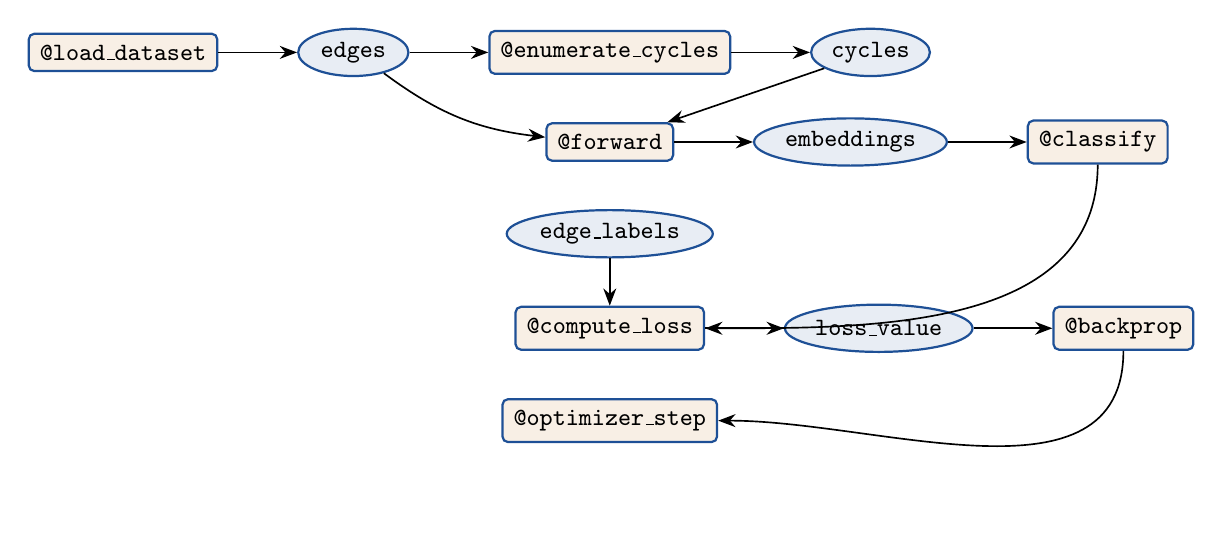
\begin{tikzpicture}[node distance=6mm and 10mm,every node/.style={font=\scriptsize}]
\node[box,fill=warn!12] (ds)  {\code{@load\_dataset}};
\node[tens,right=of ds] (e1) {\code{edges}};
\node[box,fill=warn!12,right=of e1] (cy)  {\code{@enumerate\_cycles}};
\node[tens,right=of cy] (cycs) {\code{cycles}};
\node[box,fill=warn!12,below=of cy]  (fwd) {\code{@forward}};
\node[tens,right=of fwd] (emb)  {\code{embeddings}};
\node[box,fill=warn!12,right=of emb] (cls) {\code{@classify}};
\node[tens,below=of fwd] (lbl)  {\code{edge\_labels}};
\node[box,fill=warn!12,below=of lbl] (lo) {\code{@compute\_loss}};
\node[tens,right=of lo]  (lv)  {\code{loss\_value}};
\node[box,fill=warn!12,right=of lv]  (bp) {\code{@backprop}};
\node[box,fill=warn!12,below=of lo]  (op) {\code{@optimizer\_step}};

\draw[arr] (ds)  -- (e1);
\draw[arr] (e1)  -- (cy);
\draw[arr] (cy)  -- (cycs);
\draw[arr] (cycs) -- (fwd);
\draw[arr] (e1) to[bend right=15] (fwd);
\draw[arr] (fwd) -- (emb);
\draw[arr] (emb) -- (cls);
\draw[arr] (cls.south) to[out=270,in=0] (lo.east);
\draw[arr] (lbl) -- (lo);
\draw[arr] (lo)  -- (lv);
\draw[arr] (lv)  -- (bp);
\draw[arr] (bp.south) to[out=270,in=0] (op.east);
\end{tikzpicture}
\end{center}

The \code{@compute\_loss <loss>} hyperedge carries
\code{entropy\_lambda 0.01;} as a child statement --- the driver
adds the spectral-entropy regulariser to the BCE loss when the
value is positive.

\subsection{Strategy/command pattern: cycle preprocessing}

A single hyperedge encodes the whole cycle-enumeration choice
(strategy or command, take your pick):

\begin{lstlisting}
@enumerate_cycles <cycle_enum> {
    mode          "per_vertex";
    m_per_vertex   16;
    scorer        "fraction_negative";
    pruner        "davis";        // or "balance" / "unbalanced" / "none"
    arities       [3, 4];
    (+edges, ~enumerator, -cycles);
}
\end{lstlisting}

Swapping \code{pruner} from \code{"davis"} to \code{"balance"}
without touching any other edge re-runs with the
Cartwright--Harary balanced-only filter. The driver maps these
fields to the \code{HSIKAN\_TOPK\_*} env vars consumed by
\code{n\_tuples.\_enumerate\_cycles\_fast}, which in turn calls
\code{hymeko.enumerate\_top\_k\_per\_vertex\_cycles\_signed\_rs}.

% ────────────────────────────────────────────────────────────────────
\section{Three tuning expressions}

The same architecture / training pair can be tuned three different
ways, expressed as three different policy files.

\subsection{Grid sweep (\code{sweep\_grid.hymeko})}

\begin{lstlisting}
@sweep_hidden <param_range> { target "model.hidden";       values [8, 16, 32]; }
@sweep_topk_m <param_range> { target "topk.m_per_vertex";  values [4, 16, 64]; }
@sweep_pruner <param_range> { target "topk.pruner";        values ["none", "davis", "balance"]; }
@policy <sweep_policy> { kind "full_grid"; max_runs 50; select_metric "auc"; }
\end{lstlisting}

The driver computes the Cartesian product of all
\code{<param\_range>} edges, applies each cell on top of the
\code{<param\_range>}'s \code{target} dotted-path, and runs one
training cell per point.

\subsection{Genetic algorithm (\code{sweep\_genetic.hymeko})}

Same parameter ranges, different policy:

\begin{lstlisting}
@policy <sweep_policy> {
    kind             "genetic";
    population_size   16;
    generations       10;
    elite_keep         4;
    mutation_rate      0.2;
    crossover_rate     0.6;
    ga_warmup_epochs   5;
}
\end{lstlisting}

This wires the existing \code{run\_hsikan\_genetic.py} loop ---
the GA wrapper is unchanged; only the configuration source is
\HyMeKo.

\subsection{P-graph axiom feasibility (\code{sweep\_msg.hymeko})}

This is the novel piece. Architecture choices are encoded as a
\emph{P-graph}, with the same Friedler axioms used in
\code{data/pgraph/hda.hymeko} (the chemical-process synthesis
example from earlier today):

\begin{itemize}
\item \emph{Materials} are resource budgets (GPU memory, training
      time) and the desired output (AUC).
\item \emph{Operating units} (hyperedges) are architecture choices
      that consume budget and produce quality
      (\code{cycle\_topk\_m\{4,16,64\}},
      \code{model\_h\{8,16,32\}},
      \code{train\_\{short,long\}}).
\item Each unit's edge value is its cost; the negative I/O signs
      capture which budgets it consumes.
\end{itemize}

\code{hymeko\_pgraph::lower} reads this file as a P-graph; the same
MSG / SSG / ABB pipeline picks the cost-minimum subset that
satisfies the demand for the \code{auc\_score} product node. In
effect, architecture search becomes a structural-feasibility
branch-and-bound. The 21-test \code{hymeko\_pgraph} suite proves
the lowering still works on this file (verified during the
overnight run).

% ────────────────────────────────────────────────────────────────────
\section{Driver pipeline}

\begin{center}
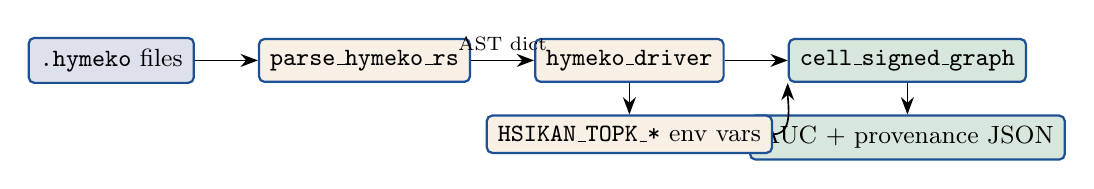
\begin{tikzpicture}[node distance=4mm and 8mm,every node/.style={font=\scriptsize}]
\node[box] (h) {\code{.hymeko} files};
\node[box,right=of h,fill=warn!12] (p) {\code{parse\_hymeko\_rs}};
\node[box,right=of p,fill=warn!12] (d) {\code{hymeko\_driver}};
\node[box,right=of d,fill=deepgreen!18] (run) {\code{cell\_signed\_graph}};
\node[box,below=of run,fill=deepgreen!18] (out) {AUC + provenance JSON};
\node[box,below=of d,fill=warn!12] (env) {\code{HSIKAN\_TOPK\_*} env vars};

\draw[arr] (h) -- (p);
\draw[arr] (p) -- node[above]{AST dict} (d);
\draw[arr] (d) -- (env);
\draw[arr] (d) -- (run);
\draw[arr] (env.east) to[out=0,in=270] (run.south west);
\draw[arr] (run) -- (out);
\end{tikzpicture}
\end{center}

\subsection{Smoke test --- \code{.hymeko} drives a real training cell}

Single-run command:
\begin{lstlisting}
python3 -m signedkan_wip.src.hymeko_driver \
    --arch     data/hsikan/arch_mixed_k34.hymeko \
    --training data/hsikan/training.hymeko \
    --dataset  bitcoin_alpha
\end{lstlisting}

Output:
\begin{lstlisting}
{"dataset": "bitcoin_alpha", "model": "HSiKAN-mixed", "hidden": 16,
 "n_test": 2420, "arities": [3, 4], "auc": 0.7930,
 "f1m": 0.4644, "fwd_per_call_ms": 20.6,
 "hymeko_arch": "HSiKAN_mixed_k34",
 "hymeko_training": {"topk_mode": "per_vertex", "topk_k": 16,
   "topk_scorer": "fraction_negative", "topk_pruner": "davis",
   "n_epochs": 30, "lr": 0.01}}
\end{lstlisting}

The \code{hymeko\_arch} and \code{hymeko\_training} fields are the
\emph{provenance trail} — every result row knows which \HyMeKo{}
description produced it.

\subsection{Sweep mode}

A 2$\times$2 micro-sweep on Bitcoin Alpha (\code{m} $\in$
\{16, 64\} $\times$ \code{pruner} $\in$ \{none, davis\}) ran end-to-end
in 2 minutes, with one JSONL row per cell:

\begin{center}
\begin{tabular}{rlrl}
\toprule
$m$ & pruner & AUC      & note \\
\midrule
16  & none   & 0.7930   & --- \\
16  & davis  & 0.7931   & davis kills $\approx 0$ triads here \\
64  & none   & 0.8481   & $+5\,$pp at $\sim 2\times$ fwd cost \\
64  & davis  & 0.8481   & --- \\
\bottomrule
\end{tabular}
\end{center}

% ────────────────────────────────────────────────────────────────────
\section{What this gives us}

\begin{enumerate}[label=(\arabic*)]
\item \textbf{One source of truth.} The architecture, training,
      and tuning are now in version-controlled \code{.hymeko}
      files instead of hand-edited \code{run\_*.py} call sites.
\item \textbf{Strategy/command pattern is a config flip.} Cycle
      enumeration is a hyperedge with a \code{pruner} field;
      changing \code{"none"} $\to$ \code{"davis"} $\to$
      \code{"balance"} requires zero code edits.
\item \textbf{Provenance.} Every trained checkpoint knows the
      exact \code{.hymeko} that produced it.
\item \textbf{Three tuning expressions, one driver.} Grid, GA, and
      P-graph axiom-feasibility all read the same arch+training
      pair; only the policy file changes.
\item \textbf{Reuses production code.} The driver wraps
      \code{run\_final\_cell.cell\_signed\_graph} and the existing
      cycle enumerator --- no parallel implementation to drift out
      of sync.
\end{enumerate}

% ────────────────────────────────────────────────────────────────────
\section{What's left}

\begin{itemize}
\item \textbf{GA driver loop} is currently scaffolded; the
      \code{<sweep\_policy kind="genetic">} branch in the driver
      needs to call \code{run\_hsikan\_genetic.py}'s evaluation
      function in place of the grid Cartesian product.
\item \textbf{MSG/SSG/ABB driver branch} should call
      \code{hymeko\_pgraph::abb\_solve} on the parsed P-graph and
      emit the optimum architecture as a synthesised
      \code{arch\_*.hymeko}.
\item \textbf{Template-side codegen} for HSiKAN is already wired
      in \code{transforms/torch\_dataflow/template.py} (Tier-3
      \code{signedkan\_layer} / \code{walk\_layer} / etc.); a
      \code{queries.hymeko}-style query for our new \code{<dataflow>}
      shape would close the codegen loop and let \code{hymeko
      compile} emit a \code{torch.nn.Module} class directly from
      \code{arch\_mixed\_k34.hymeko}.
\item \textbf{Translator-emit-back} so the driver could write a
      \code{.hymeko} for the best-found cell, completing the
      round-trip.
\end{itemize}

\end{document}
